\section{Participation notes 8}
Participant: Student.

\begin{itemize}
    \item \textbf{Have them read the code-example} - Participant did not have any problem reading the code.
    \item \textbf{Have them draw the structure} - The participant drew three Boxes the title "Main", "Hello world" and "Bye world". Within box "Hello world" and "Bye world" a general form of the implementation of the individual functions was written. In side the main box, the prticipant added two dots one above the other and drew two arrows, one from the top dot to the "Hello world" box and a second from the "Bye world" box and said this was said to represent the function calls in main. After this a line was added underneath the two dots within the box called "Main" which said "return" which was mentioned to be the return of the main function.
    \item \textbf{Have them submit the git URL} - URL submission went without problem and seemed to be intuitive.
    \item \textbf{Have them get the main() implementation} - Participant wasn't able to find implementation of both main and the other functions.
    \item \textbf{Addition notations} - Clicked the list of submitted repositories. The participants was able to scroll in/out. Participants had no problem with the camera controls.
    \item \textbf{Participant visualization} \includepdf[pages={3}]{inc/generalAppendix/userStudies/participantsVisualization.pdf}
\end{itemize}